\noindent En este sexto apartado, se busca ver como los diferentes parámetros del modelo de Heston, afectan la formula cerrada de este ultimo y las simulaciones de Monte-Carlo. Para este caso en particular, se le hizo una modificación al modelo de Monte-Carlo, donde ahora la volatilidad también sigue un proceso estocástico de la forma descrita en la ecuación \ref{volHeston}, mientras que también el precio spot sigue un proceso probabilístico, el cual ya fue descrito con anterioridad en la formula \ref{SHeston}. Por otra parte, para le ejecución de este paso, se procedió a trabajar con los primeros 100 días y el tenor de a un mes. \\ Los parámetros usados se muestran a continuación en la siguiente tabla:

\begin{table}[h]
\begin{center}
\begin{tabular}{| r | l | c |}
\hline 
Parámetros & Valores  \\ \hline
$\nu_0$ & 0.9  \\
$\Theta$ & 0.06  \\
$\omega$ & 0.02    \\
$\xi$ & 0.5   \\
$\rho$ & -0.8 \\ \hline
\end{tabular}
\caption{Parámetros iniciales Step 6}
\end{center}
\end{table}
asi también, se muestran a continuación los errores obtenidos entre los diferentes modelos:

\begin{table}[h]
\begin{center}
\begin{tabular}{| r | l | c |}
\hline 
Modelos & Errores  \\ \hline
Heston \& Black-Scholes & 135.39\% \\
Monte-Carlo y Black-Scholes & 473.37\%  \\
Heston y Monte-Carlo & 58.94\% \\ \hline
\end{tabular}
\caption{Errores entre modelos}
\label{tab:errormod}
\end{center}
\end{table}
Por otra parte y mediante la ayuda de un artículo académico, se determino el rango de valores para cada uno de los parámetros del modelo de Heston, los cuales se muestran a continuación: 
\begin{equation*}
	0\le \nu	\le1
\end{equation*}
\begin{equation*}
0	\le \Theta	\le100
\end{equation*}
\begin{equation*}
	0\le \omega	\le1
\end{equation*}
\begin{equation*}
0	\le \xi	\le0.5
\end{equation*}
\begin{equation*}
-0.9	\le \rho	\le0.9
\end{equation*}

Finalmente, se procedió a usar la metodología \textit{Ceteris-Paribus} para ver como cada uno de los diferentes parámetros afectan el valor de la opción $V_0$ al moverse entre el rango de valores ya menciona anteriormente. Los gráficos se muestran a continuación:

\begin{figure}[H]
    \begin{center}
    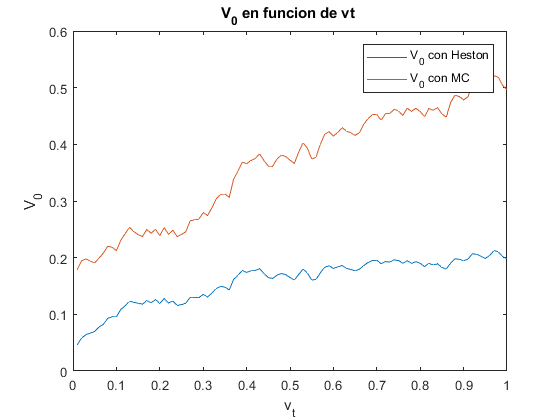
\includegraphics[width = 10cm]{figures/Paso6-1.png}
    \caption{$V_0$ en función de $\nu$}
    \end{center}
\end{figure}

\begin{figure}[H]
    \begin{center}
    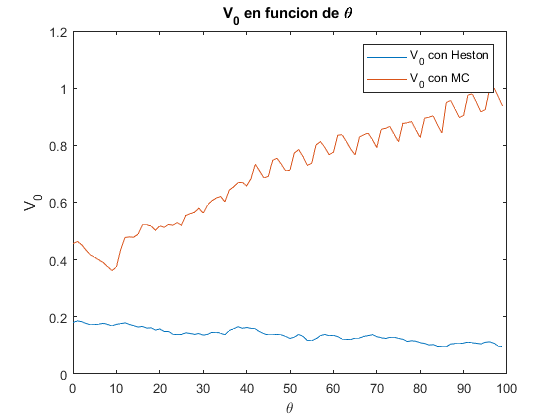
\includegraphics[width = 10cm]{figures/Paso6-2.png}
    \caption{$V_0$ en función de $\Theta$}
    \end{center}
\end{figure}

\begin{figure}[H]
    \begin{center}
    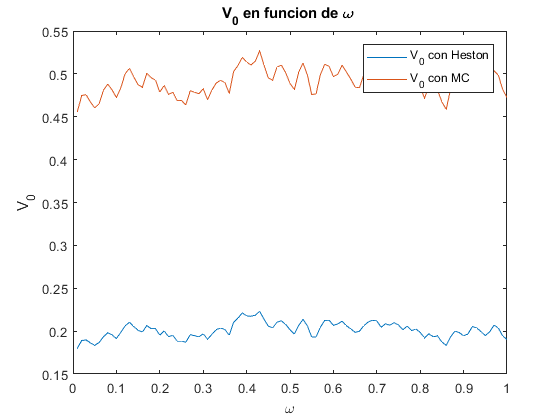
\includegraphics[width = 10cm]{figures/Paso6-3.png}
    \caption{$V_0$ en función de $\omega$}
    \end{center}
\end{figure}

\begin{figure}[H]
    \begin{center}
    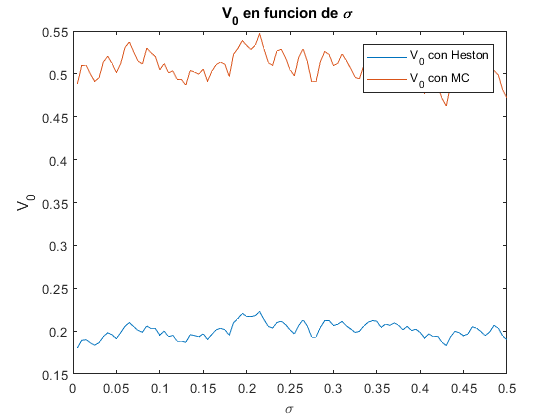
\includegraphics[width = 10cm]{figures/Paso6-4.png}
    \caption{$V_0$ en función de $\xi$}
    \end{center}
\end{figure}

\begin{figure}[H]
    \begin{center}
    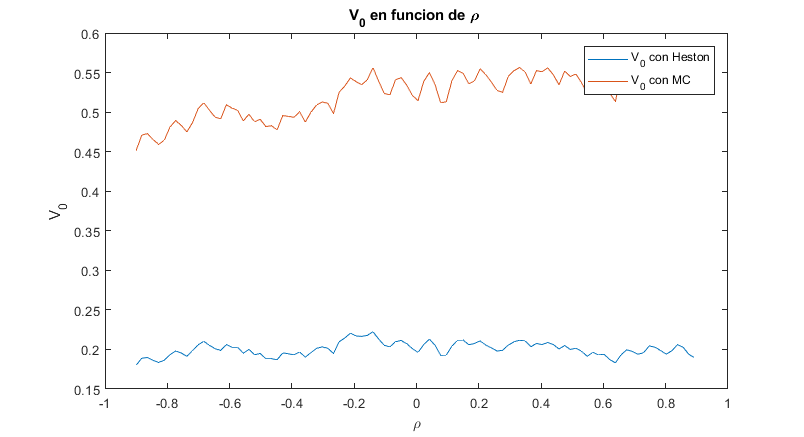
\includegraphics[width = 11cm]{figures/Paso6-5.png}
    \caption{$V_0$ en función de $\rho$}
    \end{center}
\end{figure}

De los gráficos, podemos ver como en general los valores $V_0$ no se alejan mucho entre si, a excepción de cuando  cambiamos los valores de $\nu$ y $\theta$, donde se observa que a medida que aumentamos estos, el valor de la opción tiendes a aumentar también.
\newpage
